% XeLaTeX, compile twice. Actual evidence is embedded by scripts/build_report.py.
\documentclass[UTF8,a4paper,zihao=-4,fontset=fandol]{ctexart}
\usepackage[left=25mm,right=25mm,top=24mm,bottom=24mm,headheight=15pt]{geometry}
\usepackage{graphicx,booktabs,tabularx,array,longtable,amsmath}
\usepackage[dvipsnames]{xcolor}
\usepackage{tikz}
\usetikzlibrary{arrows.meta,positioning,fit,calc}
\usepackage{caption,fancyhdr,enumitem,listings,xurl,hyperref,float,needspace,etoolbox}
\definecolor{ink}{HTML}{183C67}
\definecolor{muted}{HTML}{5C6D80}
\definecolor{pale}{HTML}{F1F5FA}
\hypersetup{unicode=true,colorlinks=true,linkcolor=ink,urlcolor=ink,
 pdftitle={表情符号课堂情绪检查器系统实验报告},pdfauthor={袁谦朗 吴卫昊 李阳 吕祖灿},bookmarksnumbered=true}
\urlstyle{same}
\graphicspath{{assets/}}
\ctexset{section={format=\Large\bfseries\color{ink},beforeskip=1.1em,afterskip=.6em},
 subsection={format=\large\bfseries,beforeskip=.8em,afterskip=.35em}}
\setlength{\parindent}{2em}
\setlength{\parskip}{.18em}
\linespread{1.25}
\setlength{\emergencystretch}{2em}
\setlength{\tabcolsep}{5pt}
\renewcommand{\arraystretch}{1.24}
\newcolumntype{Y}{>{\raggedright\arraybackslash}X}
\captionsetup{font=small,labelfont=bf,labelsep=quad,skip=6pt}
\setlist[itemize]{leftmargin=2em,itemsep=.1em,topsep=.25em}
\lstset{basicstyle=\ttfamily\footnotesize,breaklines=true,columns=fullflexible,keepspaces=true,
 backgroundcolor=\color{pale},frame=single,rulecolor=\color{ink!20},xleftmargin=.4em,xrightmargin=.4em}
\pagestyle{fancy}\fancyhf{}
\fancyhead[L]{\small 软件工程实践}
\fancyhead[R]{\small 课间晴雨\quad 课堂表情管理}
\fancyfoot[C]{\small\thepage}
\renewcommand{\headrulewidth}{0pt}
\setcounter{tocdepth}{1}
\pretocmd{\section}{\Needspace{8\baselineskip}}{}{}
\pretocmd{\subsection}{\Needspace{7\baselineskip}}{}{}
\tikzset{box/.style={draw=ink!60,rounded corners=2pt,fill=pale,align=center,
 minimum height=10mm,text width=3.4cm,font=\small},
 arrow/.style={-{Stealth[length=2mm]},draw=ink!80,semithick},
 entity/.style={draw=ink!60,rounded corners=2pt,fill=pale,align=left,text width=3.45cm,inner sep=5pt,font=\footnotesize}}
\begin{document}
\begin{titlepage}
\centering\linespread{1.1}\selectfont
\vspace*{10mm}
{\zihao{2}\heiti 中国科学技术大学\par}
\vspace{6mm}{\large 软件工程实践\par}
\vspace{23mm}
{\zihao{1}\bfseries\color{ink} 表情符号课堂\par 情绪检查器系统\par}
\vspace{8mm}{\zihao{2}\heiti 实验报告\par}
\vspace{14mm}{\large 项目名称：课间晴雨\par}
\vspace{3mm}{\large 应用场景：高新校区课堂反馈与管理\par}
\vspace{13mm}
\begin{tabular}{cc}
\toprule 小组成员 & 学号\\\midrule
袁谦朗 & PB23111711\\
吴卫昊 & PB23111689\\
李阳 & PB23050986\\
吕祖灿 & PB23111729\\\bottomrule
\end{tabular}
\vfill
源码与运行资料\par
\href{https://github.com/wwhhorizon/classroom-emoji-checker}{\nolinkurl{github.com/wwhhorizon/classroom-emoji-checker}}\par
\vspace{7mm}实验日期：2026年11月12日
\end{titlepage}
\pagenumbering{Roman}
\tableofcontents\clearpage
\pagenumbering{arabic}

\section{实验目的与系统概况}

本实验按照《表情符号课堂情绪检查器系统》实验指导书，实现一套学生、教师和管理员共同使用的课堂反馈系统。学生在课堂中选择表情，教师查看所授课程的反馈，管理员维护课堂时间和参加名单，按条件统计并导出数据。项目名称为“课间晴雨”，浏览器客户端同时适配电脑和手机，登录页采用中国科大高新校区照片。

系统包含人工反馈和视频采样两条数据路径。人工反馈保留学生主动选择的表情；视频路径按间隔抽取画面，执行人脸检测及表情分类，将达到阈值的结果写成匿名AI记录。两种来源分别统计，并共同关联到课堂会话。

工程由浏览器客户端、Web管理端、分层后端、关系数据库和独立AI服务组成。需求、设计、实现、测试、部署和演示围绕同一组课堂实体组织，形成从课堂安排到反馈查询的完整过程。实验交付包括源码仓库、数据库脚本、接口契约、测试记录、用户手册、中文解说演示及本报告。

\section{需求分析与用例建模}

\subsection{角色与数据范围}

学生负责提交和查询个人反馈，教师负责查看本人所授课堂，管理员负责课程、课堂和人员安排。AI服务使用独立身份回传推理结果，不具有用户管理权限。

\begin{table}[H]\centering\small
\caption{角色职责及访问边界}
\begin{tabularx}{\textwidth}{p{1.55cm}YY}
\toprule 角色 & 主要操作 & 数据范围\\\midrule
学生 & 注册、登录、改密、发送表情、查看历史 & 本人记录；已安排的课堂\\
教师 & 登录、改密、课堂历史、实时看板、多维统计、视频采样 & 本人所授课程与课堂\\
管理员 & 用户管理、创建课程课堂、安排名单、统计、导出、审计 & 全部课堂及用户\\
AI服务 & 人脸检测、表情分类、结果回传 & 独立服务接口；默认匿名\\
\bottomrule\end{tabularx}\end{table}

学生是否能发送表情，由身份、名单和课堂时间共同决定。教师访问某个课堂时，后端检查该课堂所属课程的教师ID。列表、统计、详情及实时连接均执行相同范围检查，避免通过直接请求接口绕过页面菜单。

\subsection{主要功能与验收条件}

\begin{longtable}{p{2cm}p{5.9cm}p{6.25cm}}
\caption{核心需求与验收条件}\label{tab:req}\\
\toprule 模块 & 功能 & 验收条件\\\midrule\endfirsthead
\toprule 模块 & 功能 & 验收条件\\\midrule\endhead
账号 & 三角色注册、登录、退出、改密 & 教师及管理员校验邀请码；改密吊销旧会话\\
课堂 & 课程教师关联，课堂起止时间、班级、教室 & 结束晚于开始；只有对应角色可管理或查看\\
名单 & 为特定课堂安排学生 & 拒绝重复、无效和非学生账号；版本冲突返回409\\
表情 & 七类选择，个人历史及分页筛选 & 已排课且课堂进行中才能提交；来源为MANUAL\\
看板 & 实时汇总、分布、分钟趋势 & 学生提交后教师无需刷新即可看到变化\\
统计 & 按课程、班级、时间段及来源筛选 & 所有图表与同一过滤范围一致\\
导出 & CSV、字段及安全转义 & 管理员权限；UTF-8 BOM；公式前缀转义\\
AI & 视频采样、人脸检测、表情分类、结果入库 & 至少五类映射；阈值过滤；独立令牌；事件幂等\\
隐私 & 内存处理，匿名AI观测 & 默认不存原图和视频，不做人脸身份识别\\
文档 & 需求、设计、API、数据库、部署、测试、手册 & 文件与实际接口和实测结果对应\\
\bottomrule\end{longtable}

\subsection{核心用例}

学生反馈用例的前置条件是账号有效、已被安排进入课堂且当前处于课堂时段。学生选择表情后，系统写入学生ID、课堂ID、表情类型、来源和时间；页面显示结果，个人历史可立即查询。

管理员排课用例先建立课程与教师关联，再创建包含时间和地点的课堂，最后选择参加学生。名单保存使用版本号，避免两个管理操作互相覆盖。已有反馈的课堂不能随意修改课程、班级和起止时间，使历史统计保持原有含义。

教师看板用例从已授权课堂进入，先取得汇总，再通过WebSocket接收更新。学生反馈与AI结果都可反映在看板中。教师可以筛选所授课程记录，其他教师的数据被后端排除。

AI采样用例由教师或管理员主动开始，视频帧经过独立推理服务，结果关联课堂后回传。无脸、低置信度或网络故障不会生成替代结果。采样结束、切换页面或离开页面时释放视频源。

\subsection{非功能需求}

安全性包括加盐密码哈希、可吊销会话、后端角色与数据范围检查、输入约束及安全导出。一致性包括名单版本更新、课堂行条件锁定和AI事件唯一约束。可维护性通过分层、模块职责及OpenAPI契约实现。可用性要求在空数据、无脸、模型故障和小屏设备上都有清楚的操作反馈。

\section{总体架构与修改版MVC}

\subsection{系统组成}

后端使用FastAPI与SQLAlchemy，浏览器使用HTML、CSS和JavaScript模块。AI采用OpenCV人脸检测与DNN推理，在独立进程中运行。关系数据库本地使用SQLite，部署提供MySQL配置和建表脚本。

\begin{figure}[H]\centering
\begin{tikzpicture}[node distance=9mm and 9mm]
\node[box] (student) {学生浏览器\\表情反馈与历史};
\node[box,right=of student] (web) {教师与管理员Web\\排课、看板与统计};
\node[box,right=of web] (ai) {独立AI服务\\检测、分类与回传};
\node[box,below=16mm of web,text width=7cm] (backend) {后端应用服务\\Controller $\rightarrow$ Service $\rightarrow$ Repository};
\node[box,below=of backend,text width=5cm] (db) {关系数据库\\MySQL部署 / SQLite本地};
\draw[arrow] (student.south) |- (backend.west);
\draw[arrow] (web) -- node[right,font=\scriptsize]{REST / WebSocket} (backend);
\draw[arrow] (ai.south) |- (backend.east);
\draw[arrow] (backend) -- (db);
\end{tikzpicture}
\caption{课堂表情系统架构}\end{figure}

浏览器不保存服务令牌，视频采样帧经后端代理转发至AI服务。独立worker可以直接读取摄像头或视频文件，调用推理接口后再向后端提交结果。AI服务只返回结构化推理结果，不直接访问业务数据库，权限、阈值和持久化由主后端统一处理。

\subsection{修改版MVC的实现}

浏览器的View负责页面和表格，Model保存界面状态并封装接口请求，Controller处理导航、表单、实时连接与采样控制。学生客户端可按MVP理解：交互控制承担Presenter职责，页面渲染和后端调用各自独立。Web管理端沿用同样的MVC模块边界。

后端Controller接收HTTP请求，Service实现排课、统计、导出和AI入库规则，Repository集中执行用户可见范围查询。身份验证和输入校验在业务操作前完成，关系实体与数据库约束定义在Model。相较服务器直接生成界面的MVC，浏览器承担视图与交互，后端通过REST提供数据；AI进一步作为独立服务接入。

\begin{table}[H]\centering\small
\caption{主要模块与代码对应}
\begin{tabularx}{\textwidth}{p{3.9cm}Y}
\toprule 文件或目录 & 职责\\\midrule
\texttt{app/main.py} & 路由、会话、角色检查、WebSocket与内存帧代理\\
\texttt{app/services.py} & 课堂版本、名单、AI事件、统计、CSV与审计\\
\texttt{app/repository.py} & 课程和课堂范围、组合筛选、时间解释\\
\texttt{app/models.py} & 实体、外键、唯一约束、枚举检查及索引\\
\texttt{app/static/} & Model、View、Controller、样式和校园照片\\
\texttt{ai\_service/} & 模型、独立API、采样worker、下载与验证\\
\bottomrule\end{tabularx}\end{table}

\section{数据模型与接口契约}

\subsection{关系实体}

Course关联授课教师；ClassSession描述某次具体课堂；ScheduleUser连接课堂与学生；EmojiRecord保存人工或AI结果。LoginSession保存会话摘要，AuditLog保存关键操作。

\begin{figure}[H]\centering
\begin{tikzpicture}[node distance=10mm and 9mm]
\node[entity] (user) {\textbf{User}\\id, username, role\\password\_hash, active};
\node[entity,right=of user] (course) {\textbf{Course}\\id, name\\teacher\_id};
\node[entity,right=of course] (session) {\textbf{ClassSession}\\id, course\_id\\start\_at, end\_at, version};
\node[entity,below=19mm of user] (schedule) {\textbf{ScheduleUser}\\session\_id, user\_id\\scheduled\_at};
\node[entity,below=19mm of course] (record) {\textbf{EmojiRecord}\\session\_id, user\_id?\\emoji, source, confidence\\timestamp, event\_id};
\node[entity,below=19mm of session] (audit) {\textbf{AuditLog / LoginSession}\\actor或user外键\\操作时间 / 会话有效期};
\draw[arrow] (user) -- node[above,font=\scriptsize]{1:N 授课} (course);
\draw[arrow] (course) -- node[above,font=\scriptsize]{1:N} (session);
\draw[arrow] (user) -- (schedule);
\draw[arrow] (session.south) -- ++(0,-7mm) -| (schedule.north);
\draw[arrow] (session.south) -- ++(0,-10mm) -| (record.north);
\draw[arrow] (user.south) -- ++(0,-12mm) -| (record.north);
\draw[arrow] (user.north) -- ++(0,8mm) -| (audit.east);
\end{tikzpicture}
\caption{核心实体关系及辅助实体}\end{figure}

User的用户名唯一，角色限定为student、teacher和admin。ScheduleUser对课堂与学生建立组合唯一约束。EmojiRecord的emoji和source有枚举检查，置信度限定在0至1之间，AI记录必须有置信度，人工记录必须有关联学生。event\_id建立唯一约束，防止网络重试重复写入。

AI默认不关联学生姓名，保存课堂、时间、设备和模型版本。系统没有人脸身份识别，因此“参与学生”只统计人工记录中的不同用户，AI数量表示采样观测次数。关系模型不包含原始视频或人脸图片字段。

\subsection{时间和一致性}

服务端业务时间统一按UTC保存，输出ISO字符串并带Z后缀，前端按上海时区展示。筛选时间必须携带时区，起止边界统一解释。AI结果还需满足当前课堂进行中、采样时间位于课堂时段且未超出有效时间窗口。

名单替换提交当前version，后端通过版本条件更新，并在同一事务中替换名单。人工反馈与AI入库在检查名单和时段前锁定课堂版本行，使其与管理员修改串行。已有反馈的课堂保留原课程、班级和时间，避免更改这些字段后历史记录被重新归类。

\subsection{主要REST接口}

\begin{longtable}{p{1.2cm}p{8.1cm}p{4.85cm}}
\caption{接口类别与权限}\\
\toprule 方法 & 路径 & 作用与权限\\\midrule\endfirsthead
\toprule 方法 & 路径 & 作用与权限\\\midrule\endhead
POST & \texttt{/api/auth/register, login, logout} & 注册、建立与吊销会话\\
PUT & \texttt{/api/auth/password} & 验证原密码并改密\\
GET & \texttt{/api/users/me} & 当前登录用户\\
GET & \texttt{/api/courses, /api/sessions} & 角色可见课程和课堂\\
POST & \texttt{/api/admin/sessions/\{id\}/schedule} & 管理员替换名单与版本校验\\
POST & \texttt{/api/emoji} & 学生提交人工表情\\
GET & \texttt{/api/emoji/history, statistics} & 分页历史与范围内汇总\\
GET & \texttt{/api/admin/dashboard/realtime} & 教师或管理员课堂看板\\
GET & \texttt{/api/admin/statistics} & 课程、班级和时间多维统计\\
GET & \texttt{/api/admin/emoji/export} & 管理员筛选导出\\
POST & \texttt{/api/ai/frame} & 任课教师或管理员内存采样代理\\
POST & \texttt{/api/ai/emoji-results} & 独立服务令牌回传AI结果\\
\bottomrule\end{longtable}

完整契约由实际应用导出为OpenAPI。普通客户端使用Session Cookie或Bearer用户令牌，AI回传使用独立服务令牌。错误统一返回code和message。教师和管理员实时看板通过\texttt{/ws/dashboard}连接，每两秒接收一次当前课堂汇总，循环中再次检查会话和权限。

\section{客户端和管理端实现}

\subsection{学生反馈与历史}

学生首页首先显示已安排课堂、起止时间、班级及教室，随后展示七个表情选项。选择后以边框和文字共同指明当前选项，发送过程中禁用按钮；提交成功后重新读取历史。未到上课时间、课堂结束或没有名单时，界面给出相应状态。

历史按权限和筛选条件分页获取，保留课程、班级、来源和时间。手机端把导航移至顶部，表情选择器换行，较宽记录表格在自身区域内滚动。表单有明确标签，按钮具有焦点样式，错误消息使用可读提示。

\begin{figure}[H]\centering
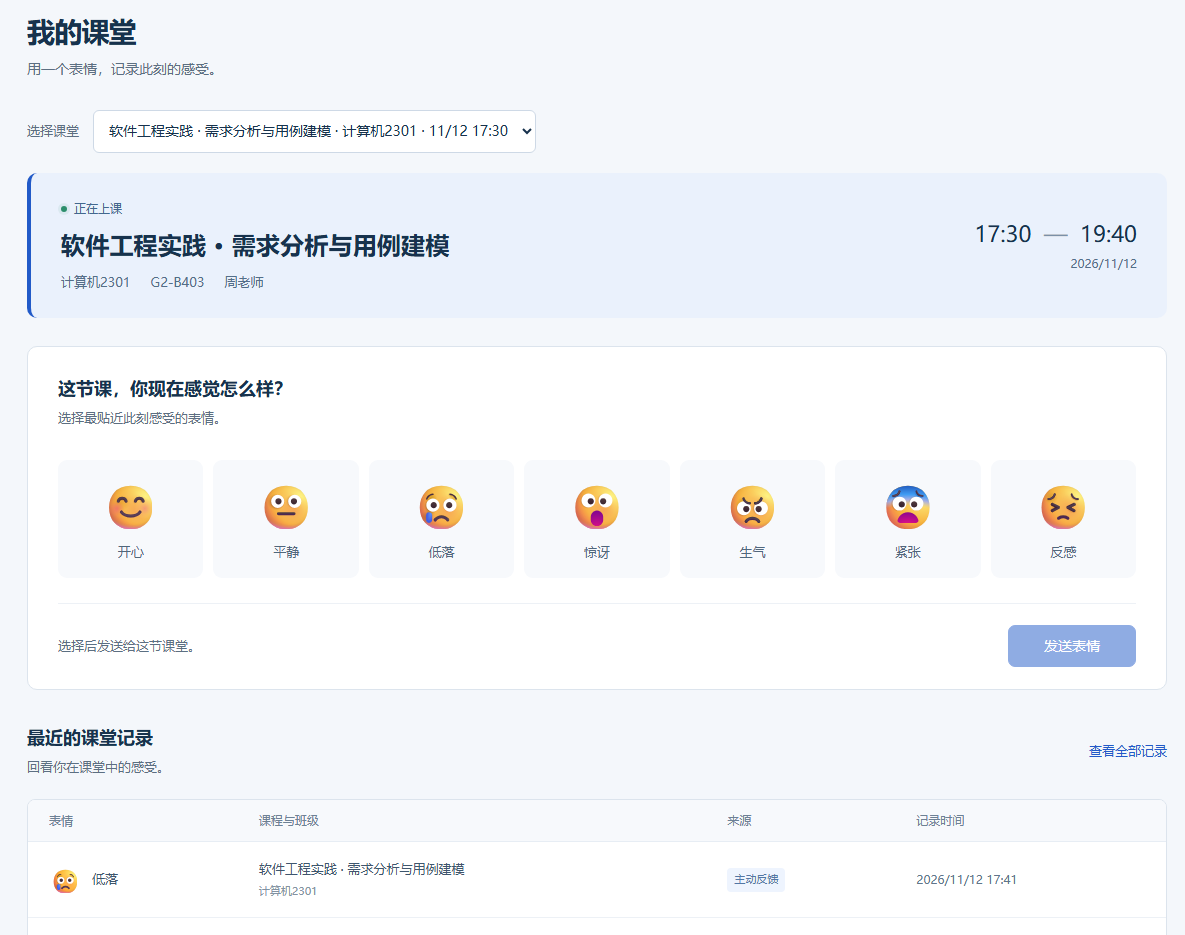
\includegraphics[width=.97\textwidth,height=.47\textheight,keepaspectratio]{student-desktop.png}
\caption{学生选择课堂表情的实际界面}\end{figure}

\subsection{课堂安排和用户管理}

管理员先创建课程并关联教师，再安排具体课堂，最后选择参加学生。名单界面直接列出有效学生，保存后可在课堂列表查看人数。版本过期时返回冲突，用户重新读取后再提交。

用户管理页面显示角色、邮箱及启用状态。停用账号同时使其已有会话失效，恢复后需要重新登录。登录、排课、名单、状态变化、表情入库及导出写入审计，管理员可以查询最近操作。

\subsection{实时看板与多维统计}

教师进入本人课堂后，看板显示表情记录数、不同学生数、主动反馈数和画面识别数。分布图展示各类数量与比例，分钟趋势仅绘制有实际记录的时间桶。切换课堂时断开旧WebSocket并创建新连接，避免前一课堂的数据写入新页面。

\begin{figure}[H]\centering
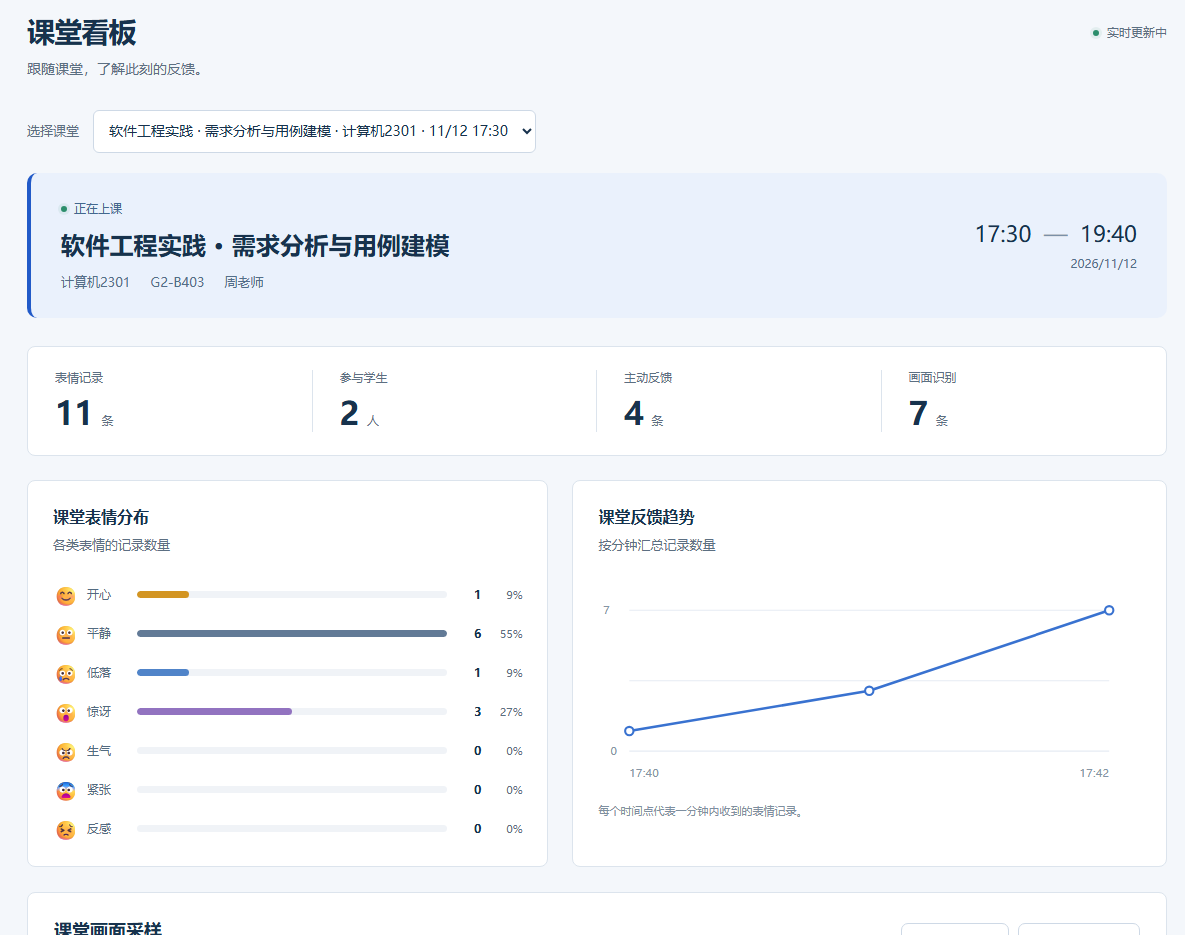
\includegraphics[width=.97\textwidth,height=.48\textheight,keepaspectratio]{teacher-desktop.png}
\caption{同一课堂中人工反馈与画面识别的教师实时看板}\end{figure}

统计分析支持课程、课堂、班级、起止时间及来源筛选，同一过滤条件用于分布、趋势、课程和班级图表。管理员导出沿用过滤范围；CSV加入UTF-8 BOM，并对可能触发表格公式的单元格前缀转义。导出事件同时保留审计记录。

\section{AI视频推理与结果入库}

\subsection{模型与预处理}

人脸检测使用OpenCV提供的正面Haar级联，表情分类采用ONNX Model Zoo的FER+模型。权重大小为35,040,571字节，通过固定SHA-256校验后加载。模型在CPU上运行，独立API接收JPEG或PNG内存字节，不依赖外部付费推理接口。

检测到的人脸转为灰度图并缩放到$64\times64$，构造$1\times1\times64\times64$的float32输入，像素保持0至255。网络输出经过稳定softmax计算概率，将contempt并入neutral后形成七类概率，再选择最大项作为结果。

\begin{table}[H]\centering\small
\caption{模型类别与系统表情映射}
\begin{tabularx}{\textwidth}{YYY}
\toprule 模型类别 & 系统枚举 & 界面含义\\\midrule
neutral、contempt & neutral & 平静\\
happiness & happy & 开心\\
surprise & surprised & 惊讶\\
sadness & sad & 低落\\
anger & angry & 生气\\
fear & fearful & 紧张\\
disgust & disgusted & 反感\\
\bottomrule\end{tabularx}\end{table}

\subsection{采样、过滤和回传}

浏览器由教师或管理员主动选择摄像头或本地视频，用Canvas按间隔抽帧，并经主后端代理送入独立AI服务。worker则直接读取摄像头或视频文件，在内存中编码JPEG，调用推理接口后回传结构化结果。

默认采样间隔为3秒，置信度阈值为0.6，均可配置。每次观测生成唯一event\_id，网络重试保持同一事件编号；后端同时检查服务令牌、课堂时间、类别、分数和事件唯一性。低分返回未接受，不增加统计。重试采用退避，无脸和服务故障保持空结果或错误提示。

浏览器代理及AI接口均按流限制请求大小，并在内存中解析multipart内容，避免普通上传接口在大文件时暂存磁盘。采样帧、解码图像和原始视频不保存，数据库只接收表情、分数、来源、课堂、设备及模型版本。

\subsection{真实推理链路验证}

本次围绕“软件工程实践：需求分析与用例建模”制作32秒课堂场景模拟视频。视频按课前准备、概念讲解、案例讨论和随堂练习编排，使用CREMA-D数据集同一成年演员的四段动态表情素材。原始绿幕被绘制的教室背景替换，画面明确标注“课堂场景模拟”及授权来源。各段完整循环播放，未根据模型输出挑选片段，素材来源、许可、哈希和合成步骤随工程保留。

在独立测试数据库中，worker采样11帧，最终新增9条AI记录，错误数为0；回传字段和课堂关联均可查询。网页端另完整播放该视频并执行采样，逐条核对识别记录与CSV导出数量。该过程验证了完整入库链路，记录保存在\texttt{docs/ai-verification.json}及演示验收文件中。

\begin{figure}[H]\centering
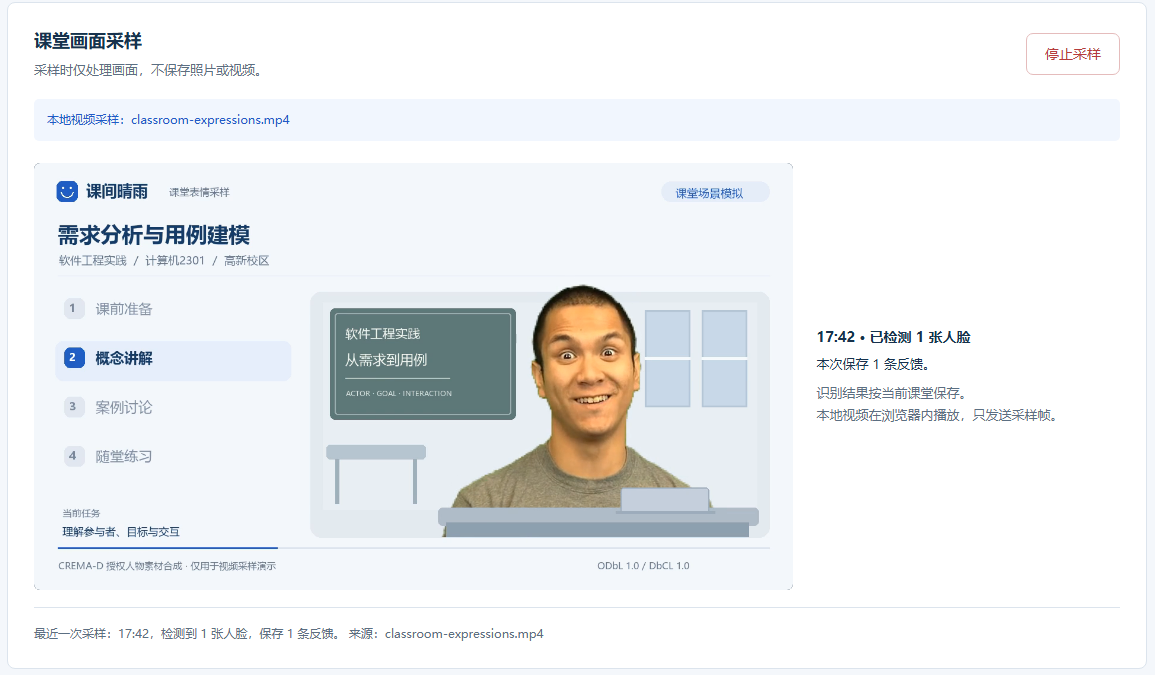
\includegraphics[width=.97\textwidth,height=.47\textheight,keepaspectratio]{ai-video-desktop.png}
\caption{本地受控视频的真实播放、采样与识别}\end{figure}

\subsection{模型局限与误判风险}

FER+未针对本校课堂重新训练。侧脸、低光照、遮挡、较小人脸以及不同群体的表情习惯会影响检测和分类；正面Haar检测对侧脸和口罩适应性有限。表情也不能直接等同于知识理解程度或心理状态，教师需要结合课堂提问、交流和学生主动反馈解释结果。

本次素材包含同一成年演员的多段表演，仍不能用它计算真实课堂准确率。逐0.5秒核验原始素材时，sad表演被模型判为neutral，anger表演多次被判为surprised；这些差异保留在素材清单中。课堂环节只是演示编排，不是情绪标签，也不能作为模型准确性的证据。后续应征得参与者同意，收集不同座位、光照和姿态的标注样本。重复采样次数不能当成独立人数，系统为此将主动反馈、画面识别和参与学生分开展示。

\section{测试设计与实际结果}

\subsection{测试环境与分层}

实际验收在Windows、Python 3.12、SQLite和Chromium环境完成。单元与接口测试使用独立数据库；浏览器验收、性能测试、AI链路和演示分别生成隔离数据库，不混入日常使用数据。测试覆盖业务Service、接口、权限、安全、WebSocket、真实AI模型及端到端流程。

\begin{table}[H]\centering\small
\caption{测试类型、重点与实际结果}
\begin{tabularx}{\textwidth}{p{2.4cm}Yp{3.1cm}}
\toprule 类型 & 验证内容 & 结果\\\midrule
单元与接口 & 账号、课堂名单、时间、版本、表情、统计、CSV、AI入库 & 51项通过，0项失败\\
安全 & 角色和课程隔离、弱密码、SQL及CSV注入、会话失效、独立令牌 & 包含于自动化测试\\
实时连接 & 学生提交后更新、越权、账号停用及会话过期 & 自动化及浏览器验证通过\\
浏览器端到端 & 注册、排课、反馈、实时查看、筛选、导出、改密 & 11阶段通过\\
可用性 & 1440像素桌面与390像素手机；标签、按钮、页面溢出 & 已核查页面无对应问题\\
AI集成 & 受控视频真实解码、采样、独立模型、匿名入库 & 11帧产生9条记录\\
演示 & 真实浏览器、中文语音和字幕、全片解码 & 时长388.98秒\\
\bottomrule\end{tabularx}\end{table}

自动化测试实际用时42.20秒。浏览器验收从零记录开始，通过界面创建课程和带时段的课堂，安排三名学生，再由两名学生生成四条人工反馈。教师页面在不刷新时从三条更新为四条；第二学生只能看到本人一条记录。管理员使用课程、班级及时间组合筛选，CSV解析后与四条记录逐一对应。

\subsection{关键异常与安全用例}

\begin{longtable}{p{3.5cm}p{6.8cm}p{3.85cm}}
\caption{代表性测试用例}\\
\toprule 场景 & 操作与预期 & 证据\\\midrule\endfirsthead
\toprule 场景 & 操作与预期 & 证据\\\midrule\endhead
名单限制 & 未排课学生提交失败；非学生和重复名单拒绝 & 后端测试\\
课堂时间 & 未开始、已结束、越界采样时间拒绝 & 后端测试\\
版本冲突 & 使用旧version修改名单返回409 & 后端测试\\
课程隔离 & teacher2读取teacher课堂返回404 & 浏览器及接口测试\\
角色隔离 & 学生访问用户管理、教师调用管理员导出返回403 & 浏览器及接口测试\\
AI阈值与去重 & 低分不入库；同事件重传不重复计数 & 后端及AI测试\\
会话安全 & 改密、停用、过期后HTTP与实时连接不能继续访问 & 后端及浏览器测试\\
图片内存处理 & 大于1MB合法帧仍不创建临时上传文件 & AI代理与服务测试\\
SQL与CSV注入 & 查询参数不能改变SQL结构；危险公式前缀转义 & 后端测试\\
真实模型 & 无脸返回空；授权动态素材使用实际FER+权重 & AI测试与链路记录\\
\bottomrule\end{longtable}

浏览器页面错误数为0。标签、按钮名称和页面横向溢出检查覆盖登录、教师看板、统计及手机学生页；这些检查与截图核对共同验证操作可读性。完整用例和JUnit结果随工程保存。

\subsection{定量性能检查}

性能脚本在新数据库中通过接口创建50条反馈，分别用1和10个并发线程执行100次已登录历史查询，每页20条。顺序请求P95为51.25毫秒，并发请求P95为251.57毫秒；相应吞吐量分别为29.34与46.32次每秒。结果仅描述本机固定数据规模下的查询，完整数值与环境保存于\texttt{docs/performance.json}。

\section{部署运行与版本管理}

\subsection{本地和容器部署}

本地入口为“启动课堂表情系统.cmd”，首次运行创建环境并检查模型，之后初始化基础账号和课堂，启动8010后端与8011独立推理服务。初始不生成表情记录；演示密码由本地配置随机生成，教师和管理员邀请码同样保存在不提交仓库的.env中。

\begin{lstlisting}
python -m venv .venv
.venv\Scripts\python.exe -m pip install -r requirements.txt -r requirements-ai.txt
.venv\Scripts\python.exe -m ai_service.download_model
.venv\Scripts\python.exe scripts/dev.py --seed
\end{lstlisting}

MySQL 8.4的建表脚本和Compose配置已提供，三个容器分别承担数据库、业务后端和AI推理；数据库使用独立卷。当前本机未安装Docker，容器和MySQL运行验收尚未完成；实际通过的运行环境为SQLite。远程CI已触发，GitHub因账号账单问题锁定而未启动任务，不能据此宣称MySQL测试通过。远程部署时应由反向代理提供HTTPS，支持WebSocket升级，并启用安全Cookie。

\subsection{测试与演示复现}

\begin{lstlisting}
python -m pytest -q
python scripts/export_contract.py
python scripts/browser_verify.py
python -m ai_service.verify_pipeline --session 1
python scripts/performance.py
python scripts/record_demo.py --dry-run
python scripts/record_demo.py
\end{lstlisting}

演示录制使用隔离数据库，先通过浏览器建立课堂和名单，再完成学生反馈、教师查看、真实视频推理和CSV导出。中文配音、字幕、逐场录屏及分镜清单一同保存，可核对每场操作和数据变化。最终视频格式为H.264/AAC，完成后检查时长和全片解码。

源码仓库为\url{https://github.com/wwhhorizon/classroom-emoji-checker}。需求基线、后端、AI、界面、验收及文档按实际工作提交，开发分支合并到主分支。仓库没有为成员补造开发时间或贡献比例。

\section{实验总结}

本项目完成了从课程与课堂安排、学生表情反馈、教师实时查看，到管理员多维统计和导出的主流程；独立视频推理通过真实模型产生匿名结果，并接入同一课堂记录体系。修改版MVC在浏览器、业务后端与AI服务之间形成明确边界，版本控制、角色范围和事件唯一约束支撑了数据一致性。

测试中较关键的处理包括课堂名单与反馈提交的并发控制、实时连接期间的会话失效、视频帧的全程内存解析，以及人工与AI统计口径的区分。这些问题分别落实到事务、循环鉴权、输入处理和页面指标中。后续工作集中于完成MySQL容器运行验收，以及在有授权和标注的课堂样本上评估模型表现。

\clearpage
\appendix
\section{提交材料索引}
\begin{longtable}{p{4.5cm}p{9.65cm}}
\toprule 材料 & 位置\\\midrule\endfirsthead
\toprule 材料 & 位置\\\midrule\endhead
需求及验收对照 & \texttt{docs/requirements.md, traceability.md}\\
设计与修改版MVC & \texttt{docs/design.md}及本报告第三、四节\\
API与数据库 & \texttt{docs/api.md, docs/openapi.json, database/schema.sql}\\
测试用例与实际记录 & \texttt{tests/, docs/testing.md, docs/verification.json}\\
部署与用户手册 & \texttt{docs/deployment.md, docs/user-manual.md}\\
AI说明与真实链路 & \texttt{docs/ai-model.md, docs/ai-verification.json}\\
视频与可编辑素材 & \texttt{deliverables/}及\texttt{demo-source/}\\
LaTeX及图片资源 & \texttt{deliverables/latex-report/report.tex, assets/}\\
源码仓库 & \url{https://github.com/wwhhorizon/classroom-emoji-checker}\\
\bottomrule\end{longtable}
\end{document}
